\chapter{Discussion}

\section{Dataset diversity}
\label{dataset_divers}
As mentioned in chapter \ref{sec:test_on_trf}, Yolo performs almost perfectly on the Trondheimsfjorden dataset, which could be an indication of overtraining. The Trondheimsfjorden dataset consists of approximately 500 images taken in the Trondheimfjord during a ferry trip back and forth between Trondheim and Brekstad. The images were all captured the same day, under the same weather and lighting conditions. Also, due to a limited amount of boats at sea during the ferry trip, multiple images were captured of the same boats. Thus even though the images the detection models were tested on and trained on were separated, the images used in both testing and training had some common features. While this might give the impression that the results are biased, and not representative of how the algorithm would perform in a completely new environment, some arguments would suggest otherwise.

\vspace{3mm}

\noindent
First of all, as shown in chapter \ref{sec:moored_boats}, Yolo$_{\text{BSM}}$ and Yolo$_{\text{BSMH}}$ perform better than Yolo$_{\text{BS}}$ on the Trondheimsfjorden test set. All these detection models are trained on datasets BoatsClose, BoatsFar and Trondheimsfjorden, while Yolo$_{\text{BSM}}$ and Yolo$_{\text{BSMH}}$ are also trained on other datasets that do not contain similar images as Trondheimsfjorden. This could imply that what improves the results of Yolo$_{\text{BSM}}$ and Yolo$_{\text{BSMH}}$ on Trondheimsfjorden, is not overtraining on the Trondheimsfjorden dataset, but rather the ability to recognize features in more diverse environments. 

\vspace{3mm}
\noindent
All the Yolo models has less accurate results on the BoatsClose and BoatsFar test set compared to Trondheimsfjorden. In BoatsClose on BoatsFar Yolo gets good results on images that contain separated boats, similar to the photos in the Trondheimsfjorden dataset. What makes the results less impressing are primarily due to images that include clusters of small boats, as shown in figure \ref{fig:yolo3_clutter}. 

\begin{figure}[h!]
\begin{subfigure}{.5\textwidth}
  \centering
  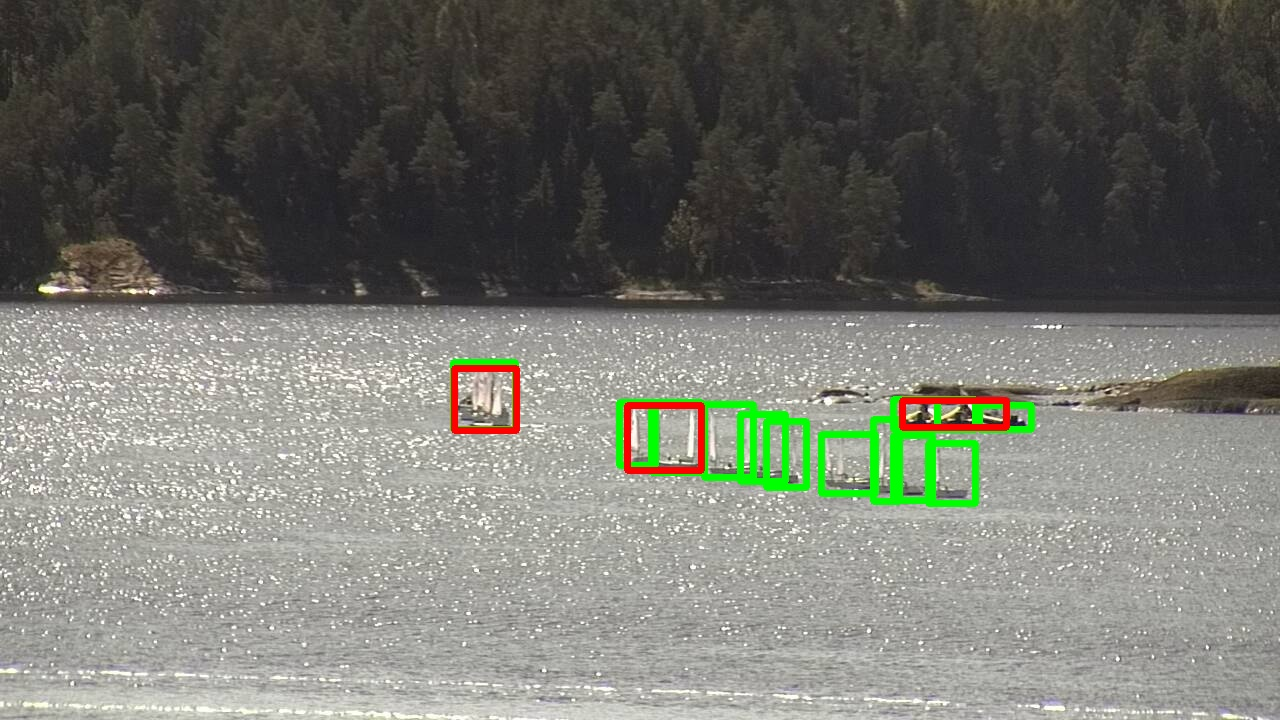
\includegraphics[width=0.8\linewidth]{discussion/clutter_yolo3/selected_08_10_frame0130.jpg}
  %\caption{Yolo$_{\text{BSMH}}$ on cluttered small boats}
  %\label{fig:yolo1_multibox}
\end{subfigure}%
\begin{subfigure}{.5\textwidth}
  \centering
  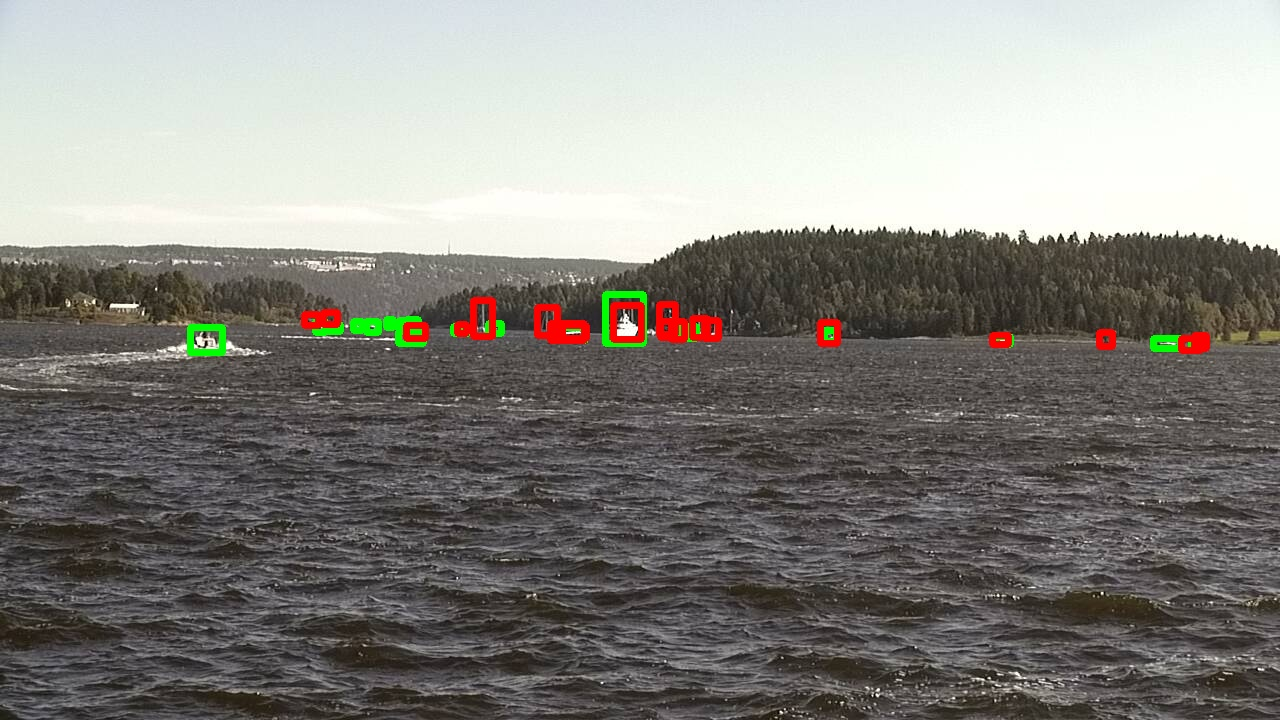
\includegraphics[width=.8\linewidth]{discussion/clutter_yolo3/selected_08_11_frame6630.jpg}
  %\caption{Yolo$_{\text{BSMH}}$ on clu}
  %\label{fig:yolo2_multibox}
\end{subfigure}
\caption{Yolo$_{\text{BSMH}}$ on cluttered small boats, red bounding boxes are detections, green bounding boxes are ground truth.}
\label{fig:yolo3_clutter}
\end{figure}

\newpage

\noindent
In the majority of the images, Yolo$_{\text{BSMH}}$ also gets excellent results in this test set, as shown in figure \ref{fig:yolo3_good_ex}.

\begin{figure}[h!]
\begin{subfigure}{.5\textwidth}
  \centering
  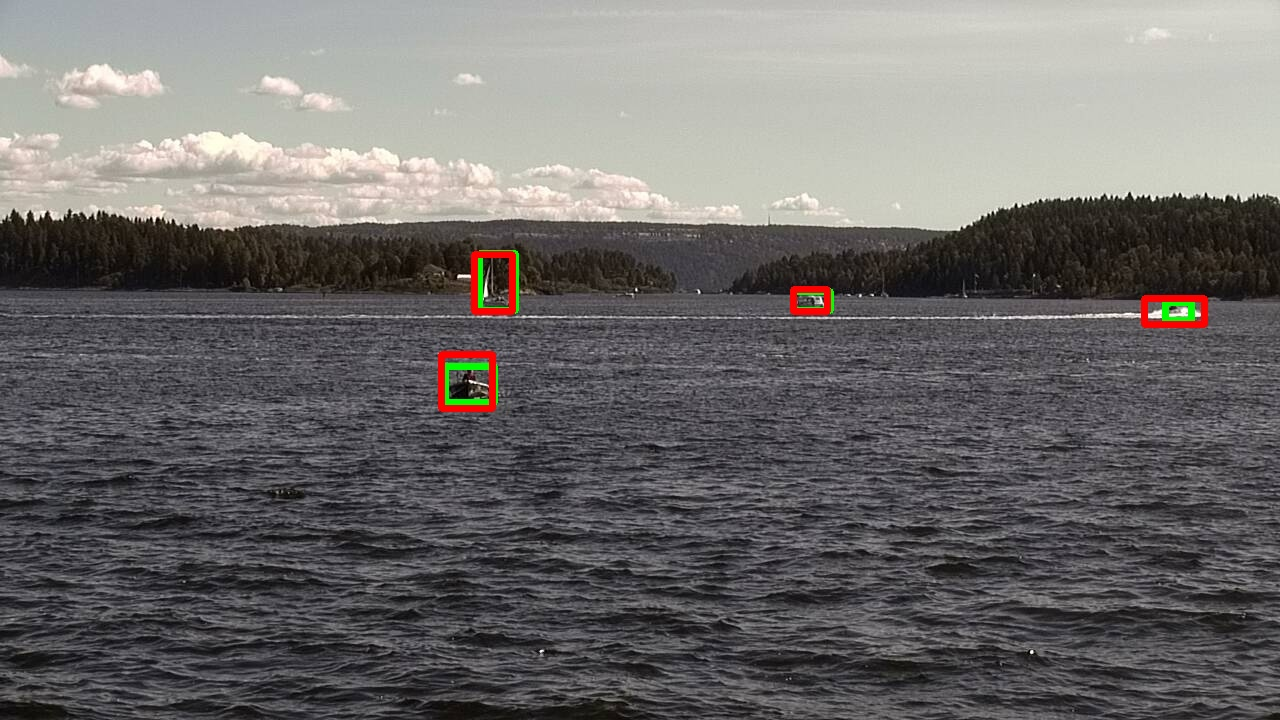
\includegraphics[width=0.8\linewidth]{discussion/good_ex/selected_08_14_frame1140.jpg}
  %\caption{Yolo$_{\text{BSMH}}$ on cluttered small boats}
  %\label{fig:yolo1_multibox}
\end{subfigure}%
\begin{subfigure}{.5\textwidth}
  \centering
  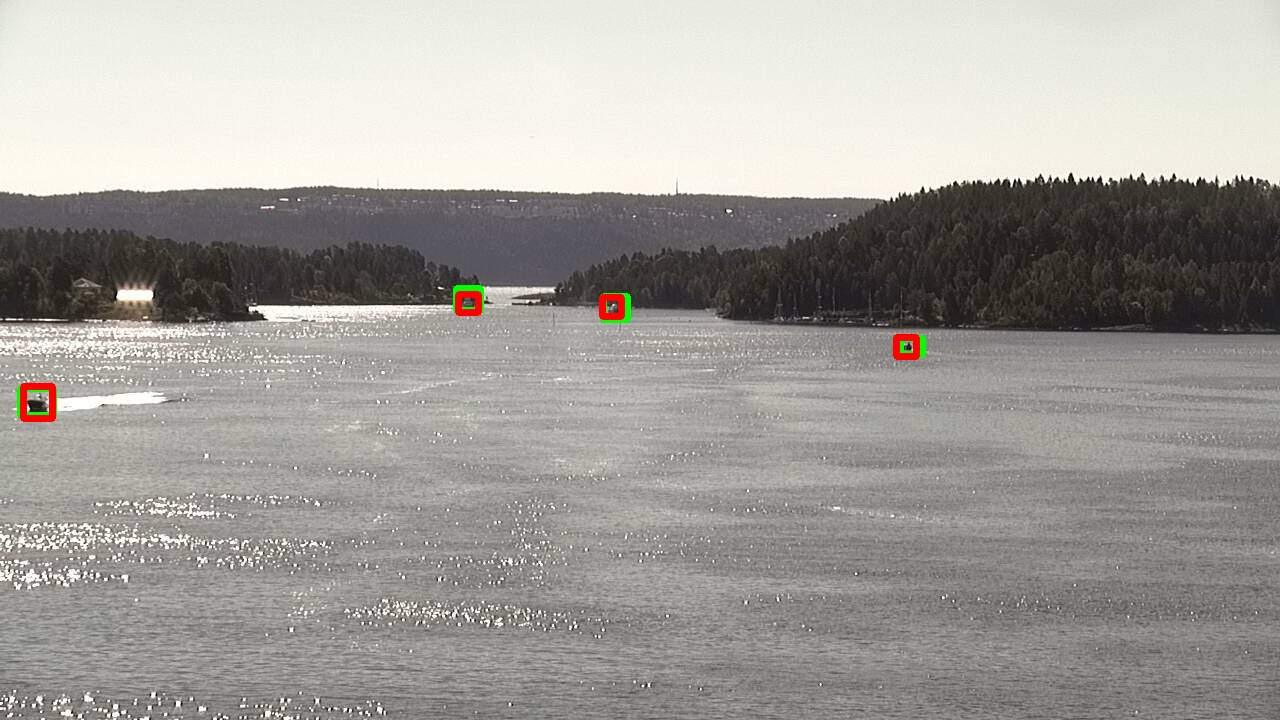
\includegraphics[width=.8\linewidth]{discussion/good_ex/selected_08_11_frame1380.jpg}
  %\caption{Yolo$_{\text{BSMH}}$ on clu}
  %\label{fig:yolo2_multibox}
\end{subfigure}
\caption{Yolo$_{\text{BSMH}}$ on separated boats in BoatsClose BoatsFar, red bounding boxes are detections, green bounding boxes are ground truth.}
\label{fig:yolo3_good_ex}
\end{figure}

\noindent
In the images in figure \ref{fig:yolo3_clutter} it is not easy to correctly detect all the boats by human assessment either. When boats are separated, Yolo$_{\text{BSMH}}$ gets good results consistently. When vessels are more prominent, cluttering does not seem to be as problematic. This could partly be because big ships do not tend to stay very close together, and thus, the examples are fewer. An example of how Yolo$_{\text{BS}}$ handles three big tow boats close together is shown in \ref{fig:yolo1_clutter}.

\begin{figure}[h!]
\begin{subfigure}{.5\textwidth}
  \centering
  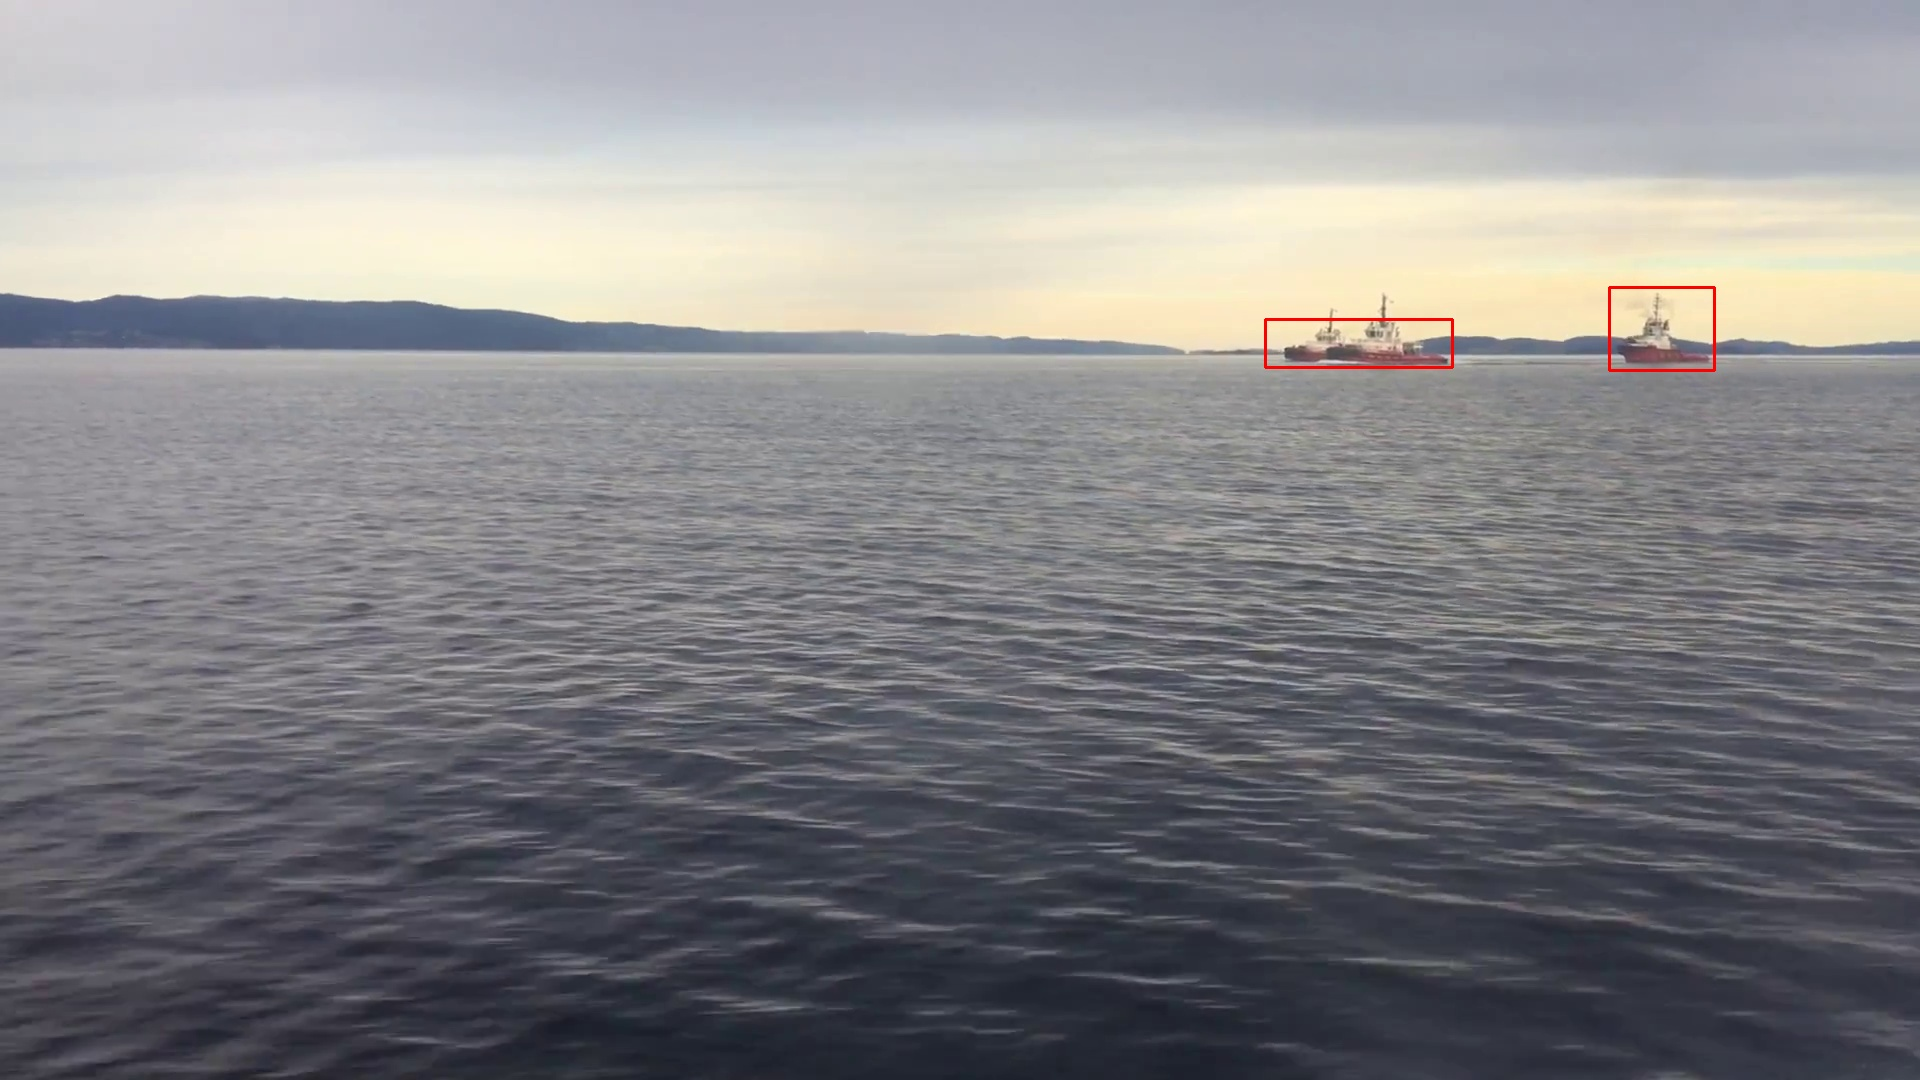
\includegraphics[width=0.8\linewidth]{results/video/video3/frame479.jpg}
  \caption{One tow boat partly covered by another.}
  \label{fig:yolo1_clut_tow}
\end{subfigure}%
\begin{subfigure}{.5\textwidth}
  \centering
  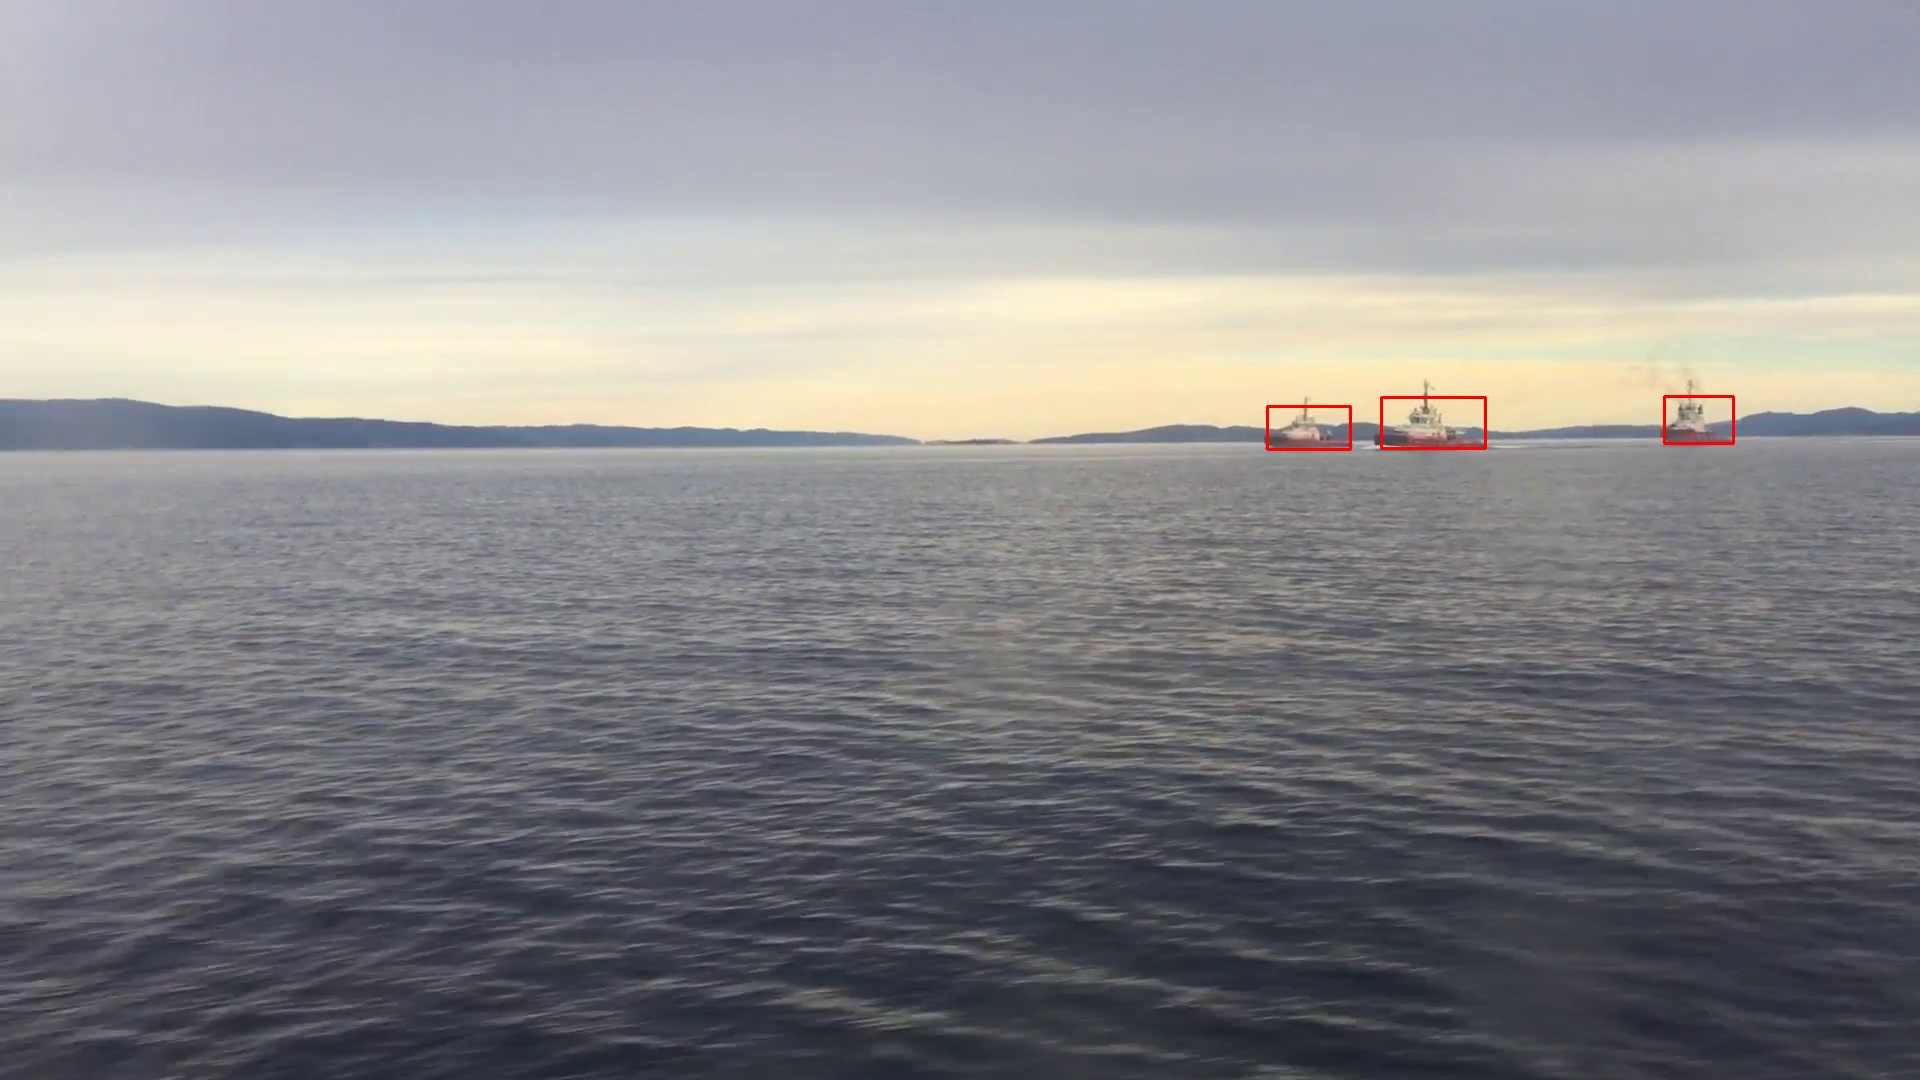
\includegraphics[width=.8\linewidth]{results/video/video3/frame677.jpg}
  \caption{Three tow boats separated.}
  \label{fig:yolo1_sep}
\end{subfigure}
\caption{Yolo$_{\text{BS}}$ on big boat clutter, red bounding boxes are detections, green bounding boxes are ground truth.}
\label{fig:yolo1_clutter}
\end{figure}

\noindent
In both figure \ref{fig:yolo1_clut_tow} and \ref{fig:yolo1_sep} there are three towboats. In figure \ref{fig:yolo1_clut_tow} one of the boats is partly covered by another, and the two boats are detected as one. This is not necessarily a problem, and as soon as the boats are separated, they are detected as three boats. 

\vspace{3mm}

\noindent
One cannot rule out that the results are unaffected by overtraining. To verify if the detection model is overtrained or not one would have to evaluate it in completely unseen environments. At the same time, it does not serve any purpose to test the detection algorithm on a dataset that is nothing alike the Trondheimsfjorden dataset, since this is the environment the algorithm is meant to perform well in. The Trondheimsfjorden dataset contains many different types of boats and ships, it contains large camouflaged military vessels, small motor boats, and ferries, and is diverse relative to how different the boats and ships in the Trondheimfjord generally is. 

\vspace{3mm}

\noindent
The accuracy of the results Yolo$_{\text{BSMH}}$ has on the Trondheimsfjorden test set might also be because the detection problem of maritime vessels in the Trondheimfjord is not where Yolo struggles. It will depend on each case, but the results in this project indicate that Yolo can robustly detect sailing boats in the Trondheimfjord under good weather conditions. To verify this claim one would need an even more diverse test set, to ensure that the good results are not a consequence of overtraining. Still, there is no limit to how diverse a dataset could be and building a dataset that could verify this claim one hundred percent seems like an impossible task. 

\vspace{3mm}
\noindent
That being said, the weather conditions do not vary much, neither in the test or training dataset. Ideally, a dataset with a diverse set of ships and boats under different weather conditions such as dark lighting conditions, fog and snow should be made. The Cloud Detection Framework can be easily used to address the different scenarios, but the compilation of a dataset for these conditions should be done in future research on this topic.






\newpage

\subsection{Non-detected buildings in Trondheimsfjorden}
\label{sec:build_trf}
In the Trondheimsfjorden dataset, there are buildings in the background which Yolo$_{\text{BSMH}}$ does not detect, even though it is trained on a building class. The building dataset contains images taken in Trondheim close to Nidelva and a canal, and the buildings are in the majority of the images close up, as shown in figure \ref{fig:buildings}

\begin{figure}[h!]
\begin{subfigure}{.5\textwidth}
  \centering
  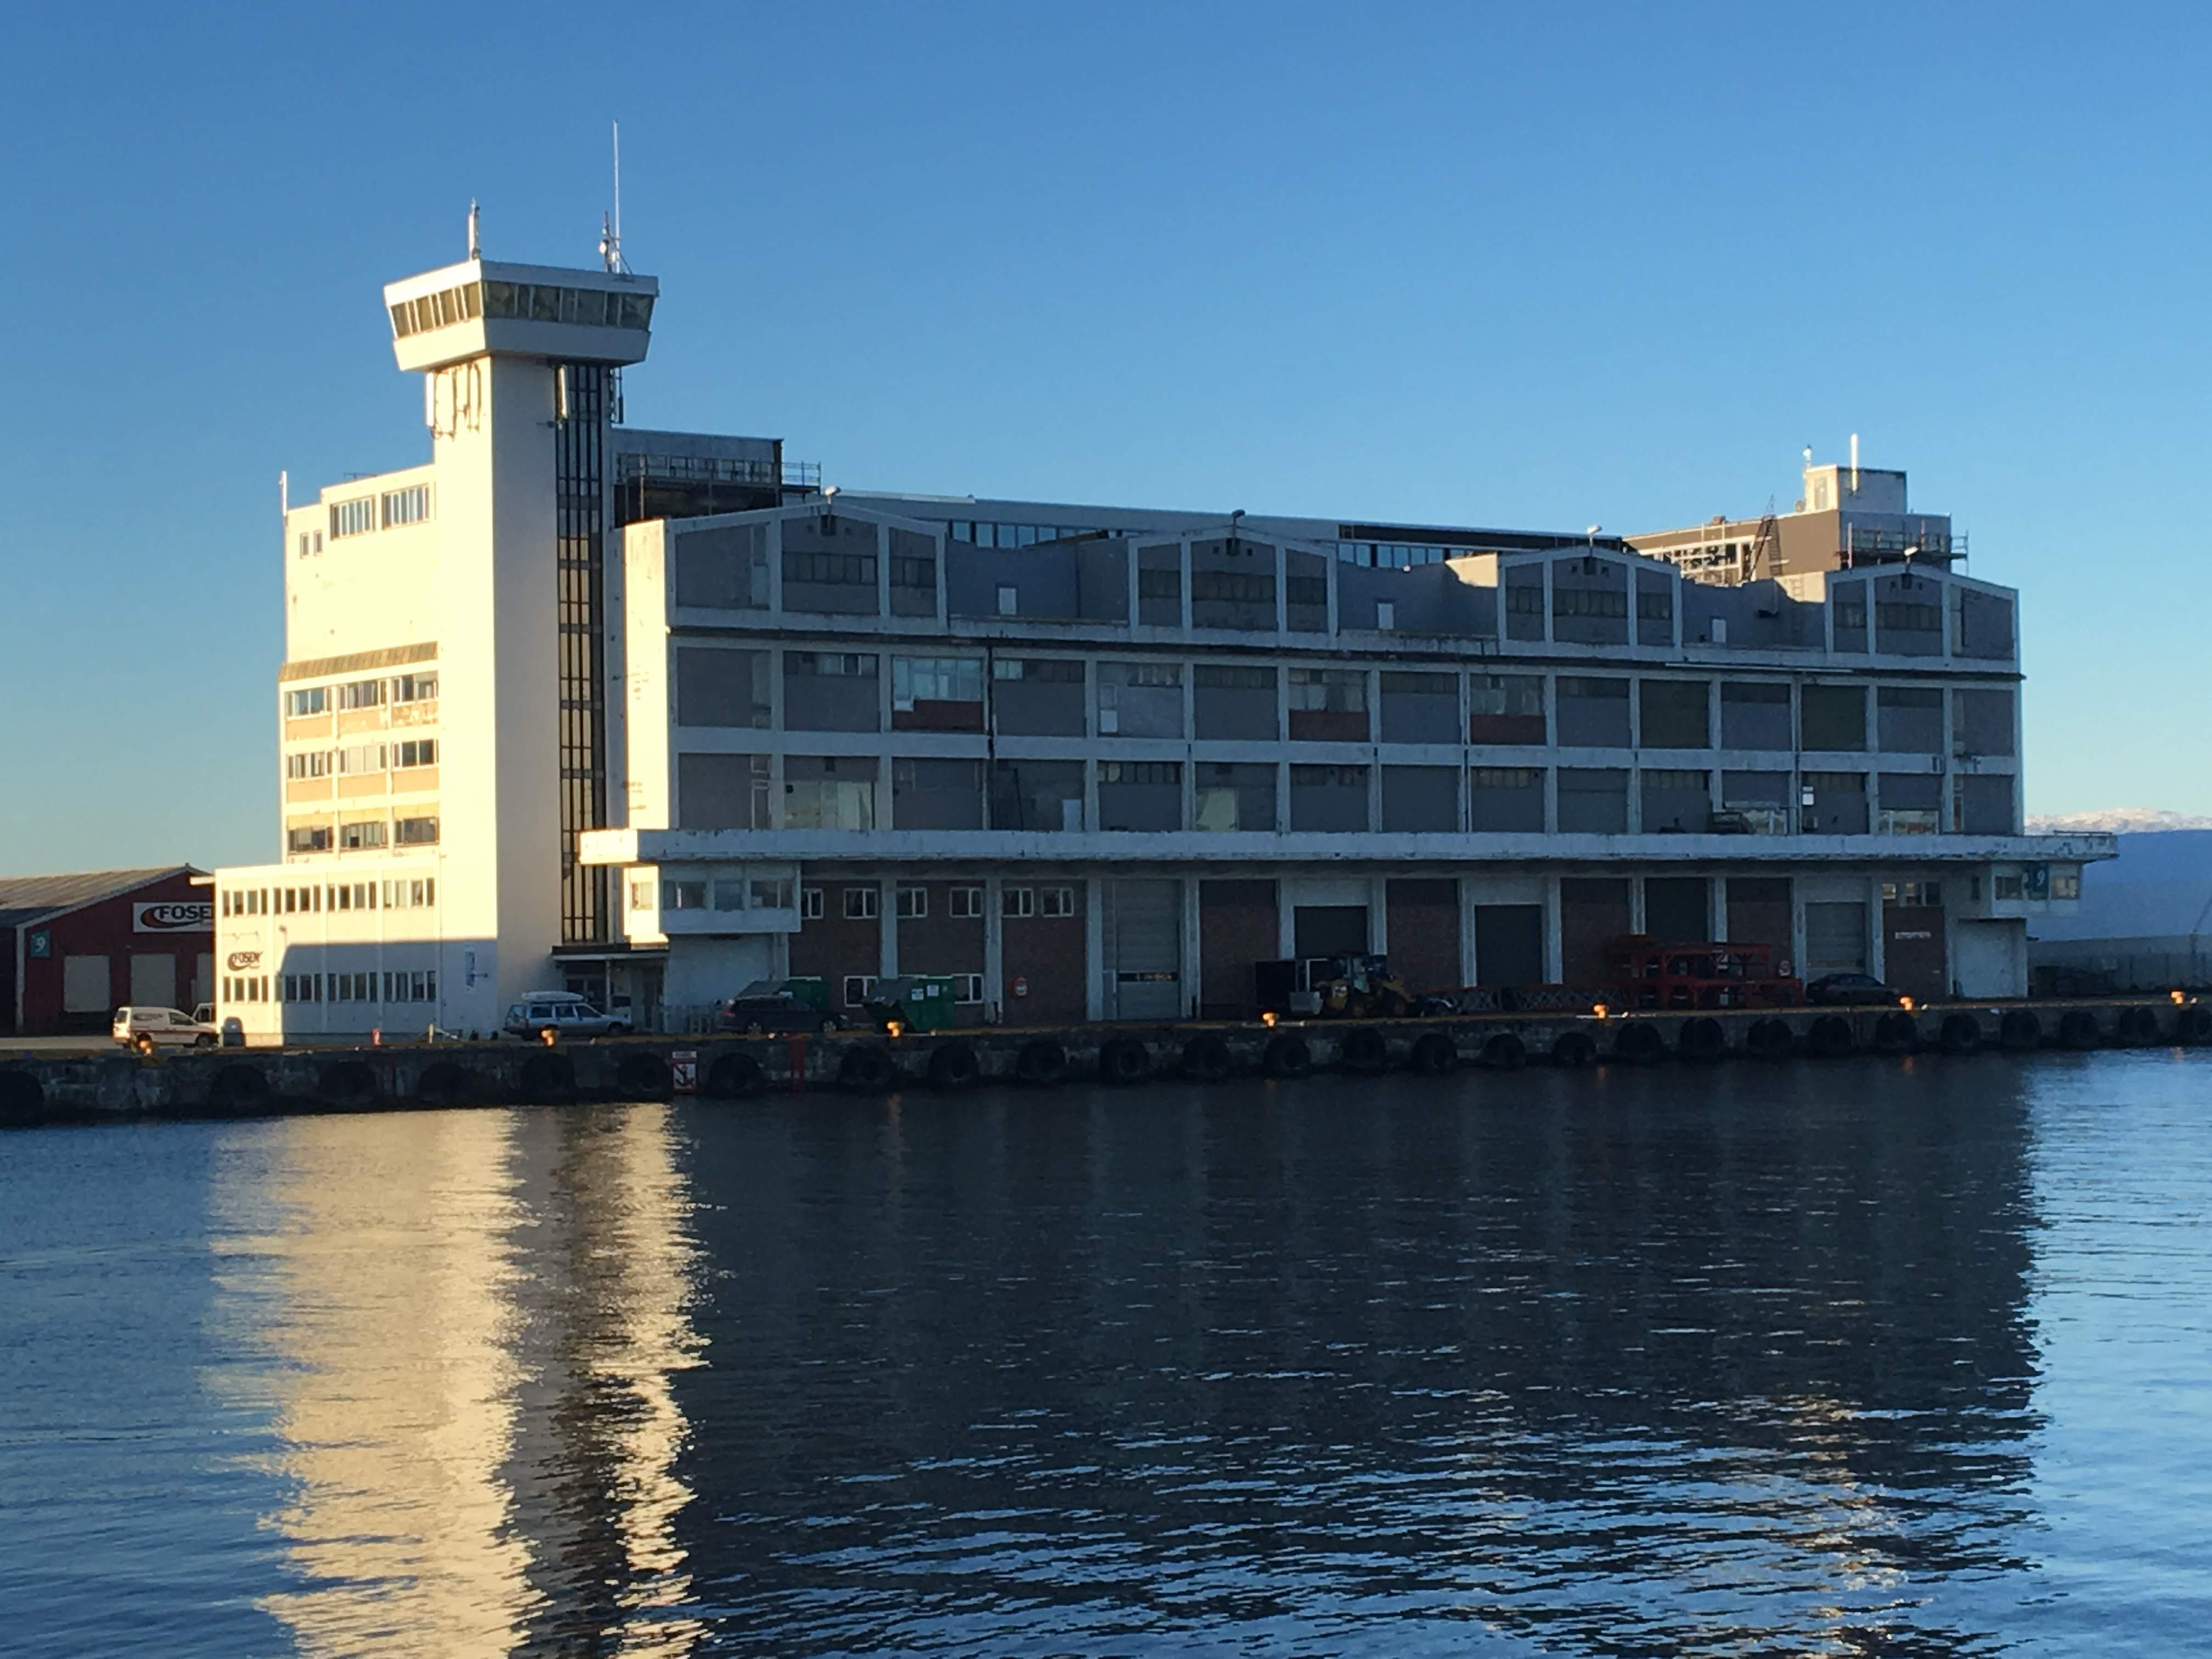
\includegraphics[width=0.8\linewidth]{discussion/buildings/IMG_2136.jpg}
  %\caption{One tow boat partly covered by another}
  %\label{fig:yolo1_clut_tow}
\end{subfigure}%
\begin{subfigure}{.5\textwidth}
  \centering
  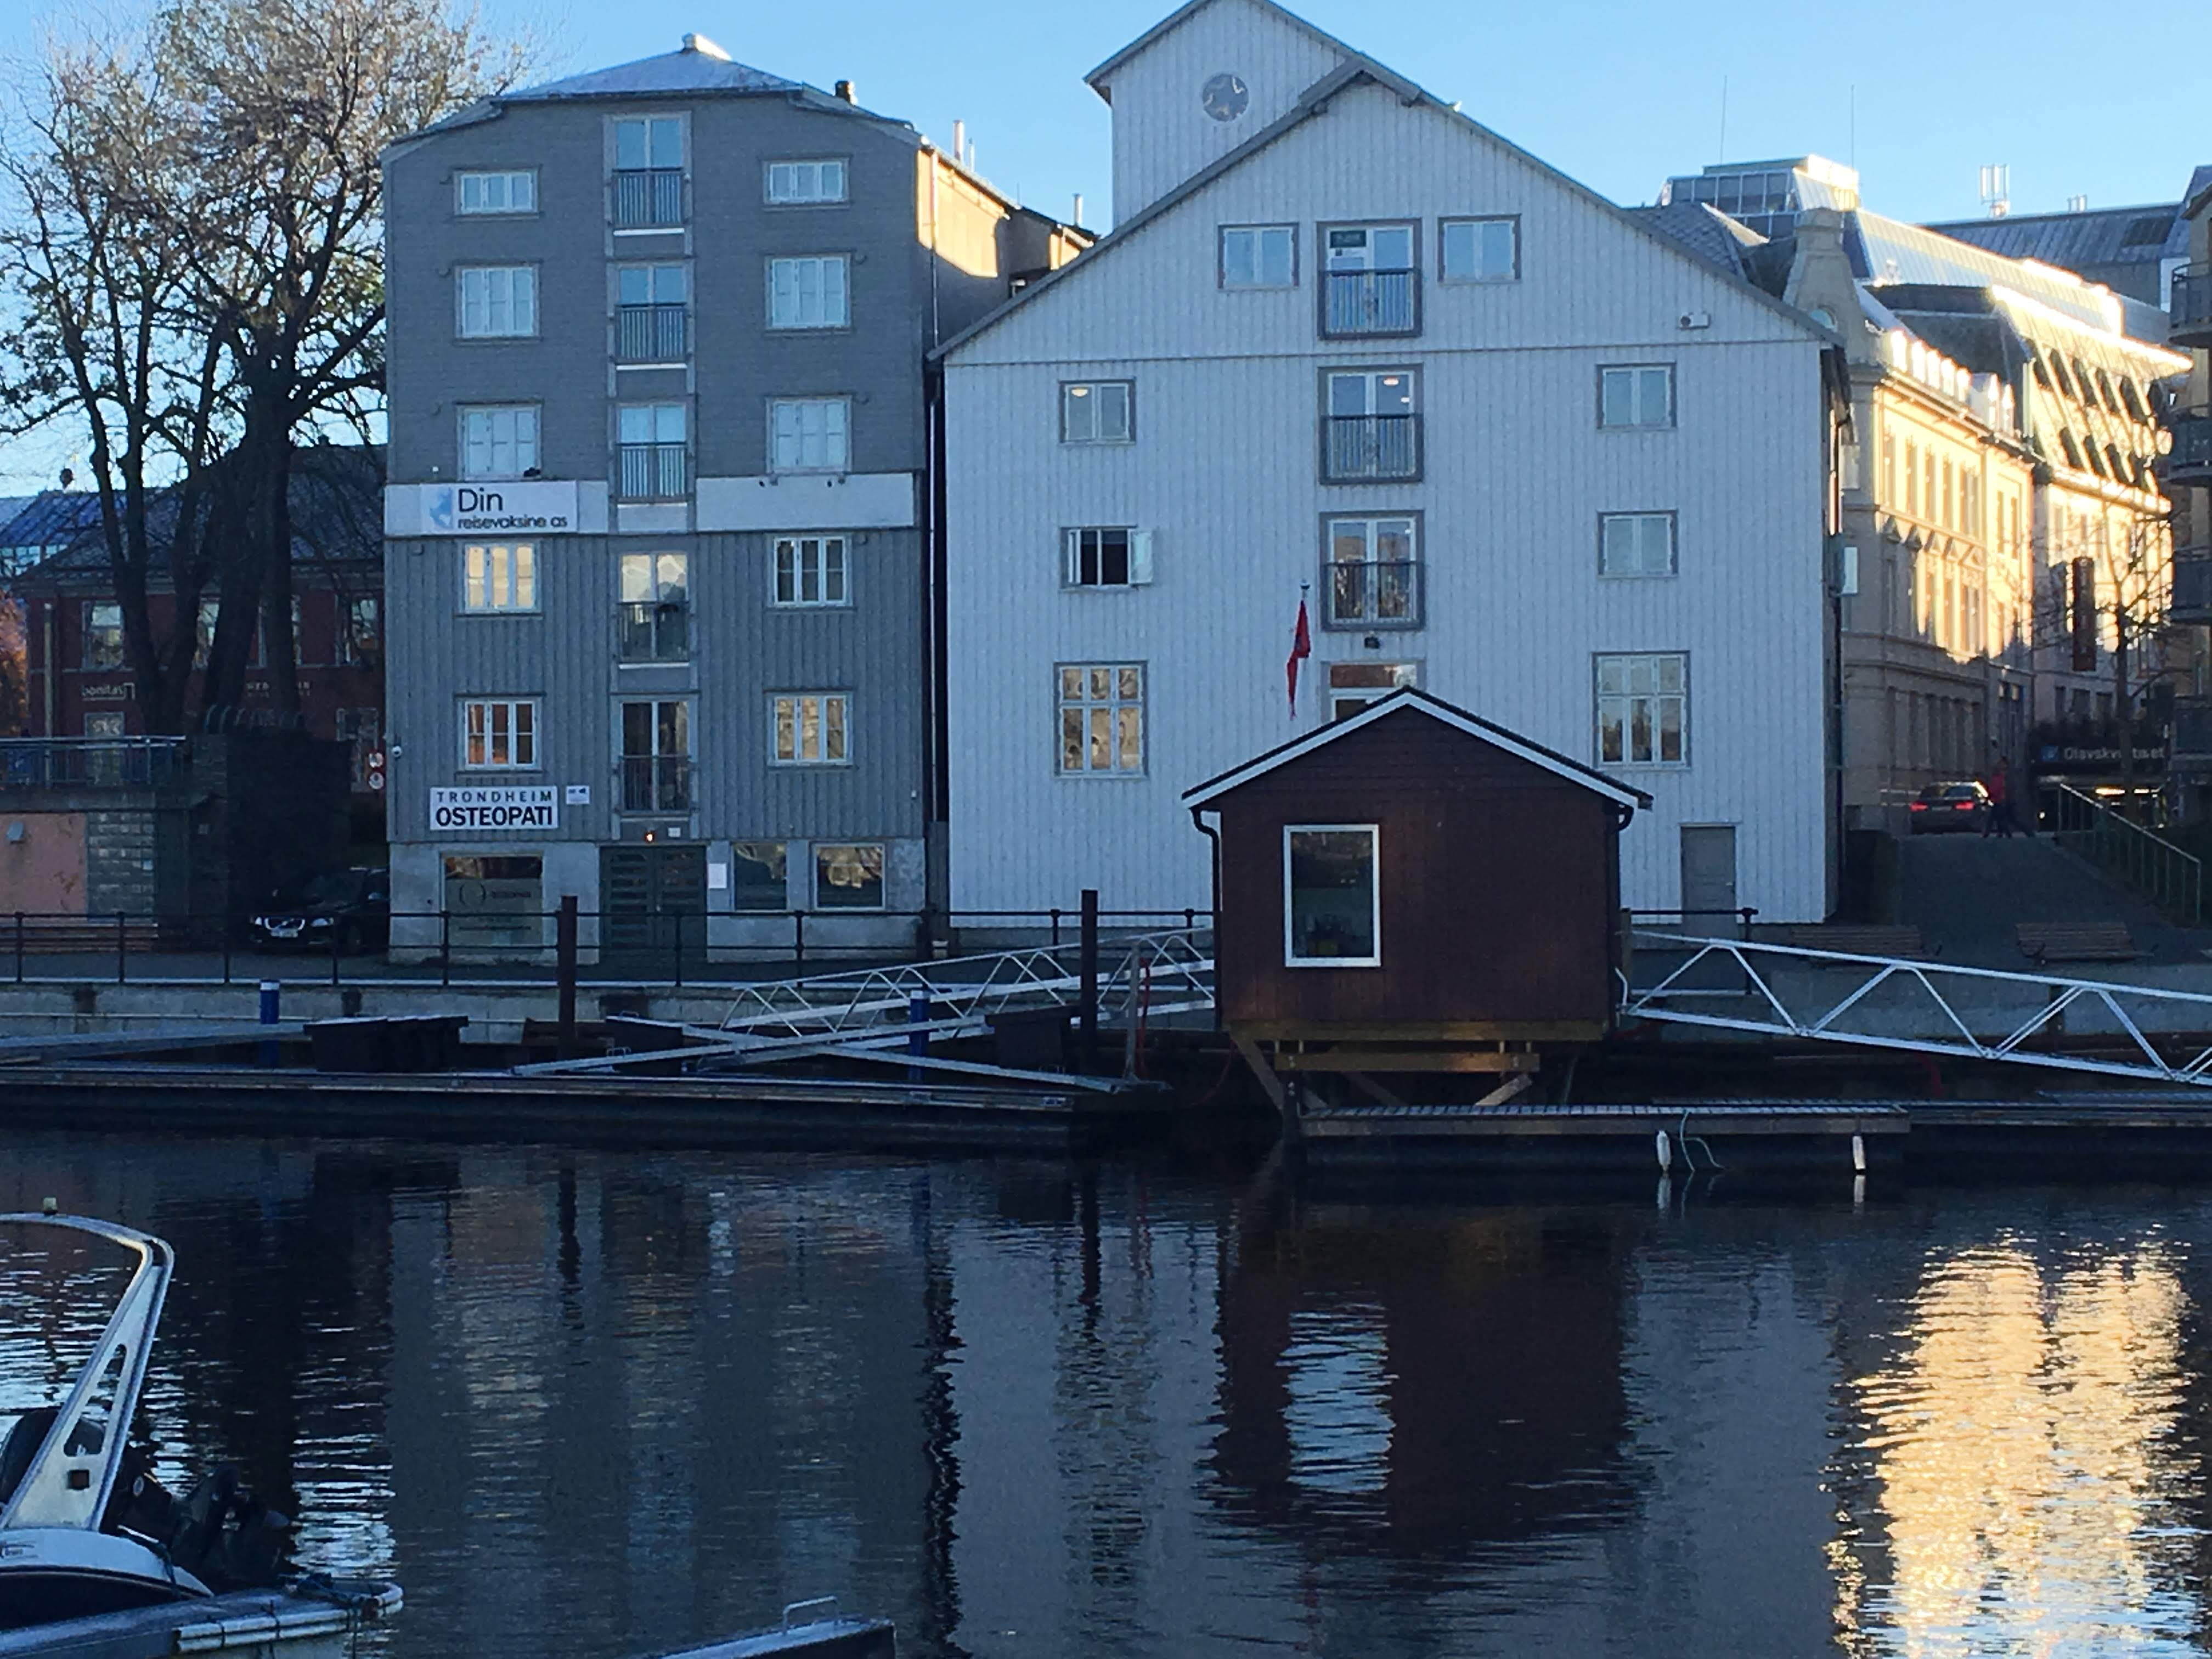
\includegraphics[width=.8\linewidth]{discussion/buildings/IMG_2085.jpg}
  %\caption{Three tow boats separated}
  %\label{fig:yolo1_sep}
\end{subfigure}
\caption{Example images from the buildings dataset.}
\label{fig:buildings}
\end{figure}

\noindent
In Trondheimsfjorden, there are examples where Yolo$_{\text{BSMH}}$ fails to detect buildings, as shown in figure \ref{fig:yolo3_no_build}.

\begin{figure}[h!]
\begin{subfigure}{.5\textwidth}
  \centering
  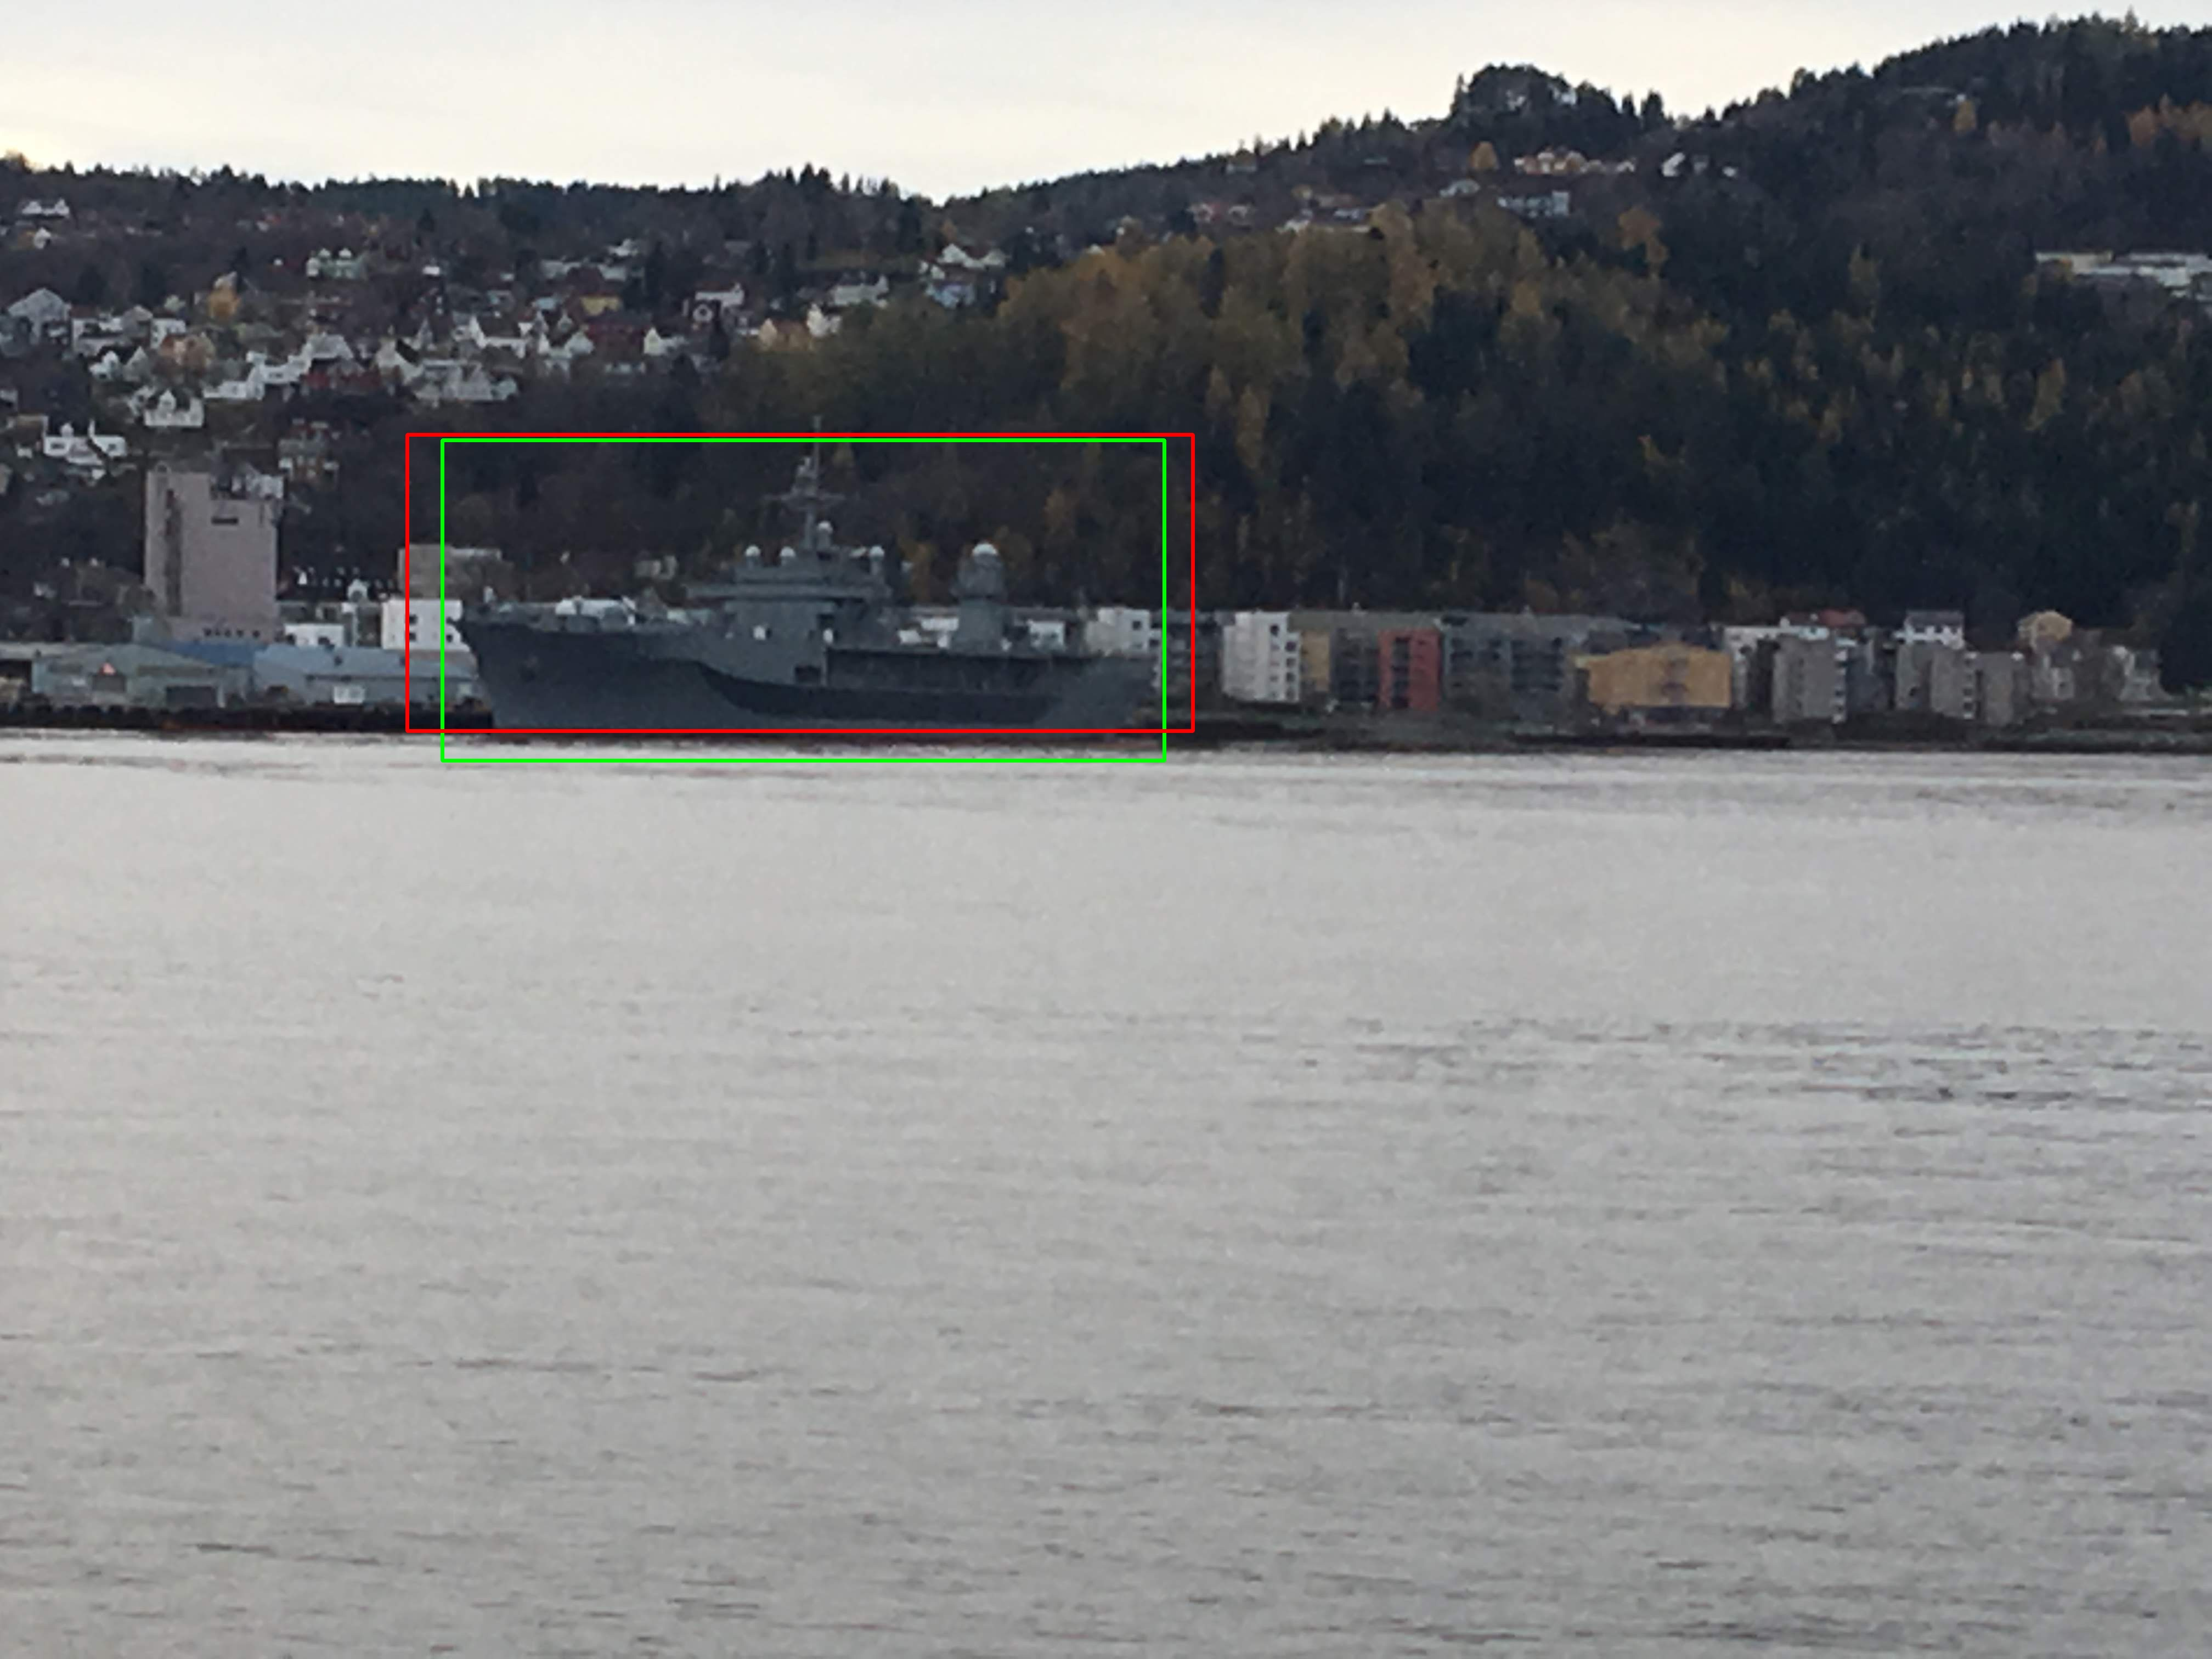
\includegraphics[width=0.8\linewidth]{discussion/yolo3_no_build/IMG_2673.jpg}
  %\caption{One tow boat partly covered by another}
  %\label{fig:yolo1_clut_tow}
\end{subfigure}%
\begin{subfigure}{.5\textwidth}
  \centering
  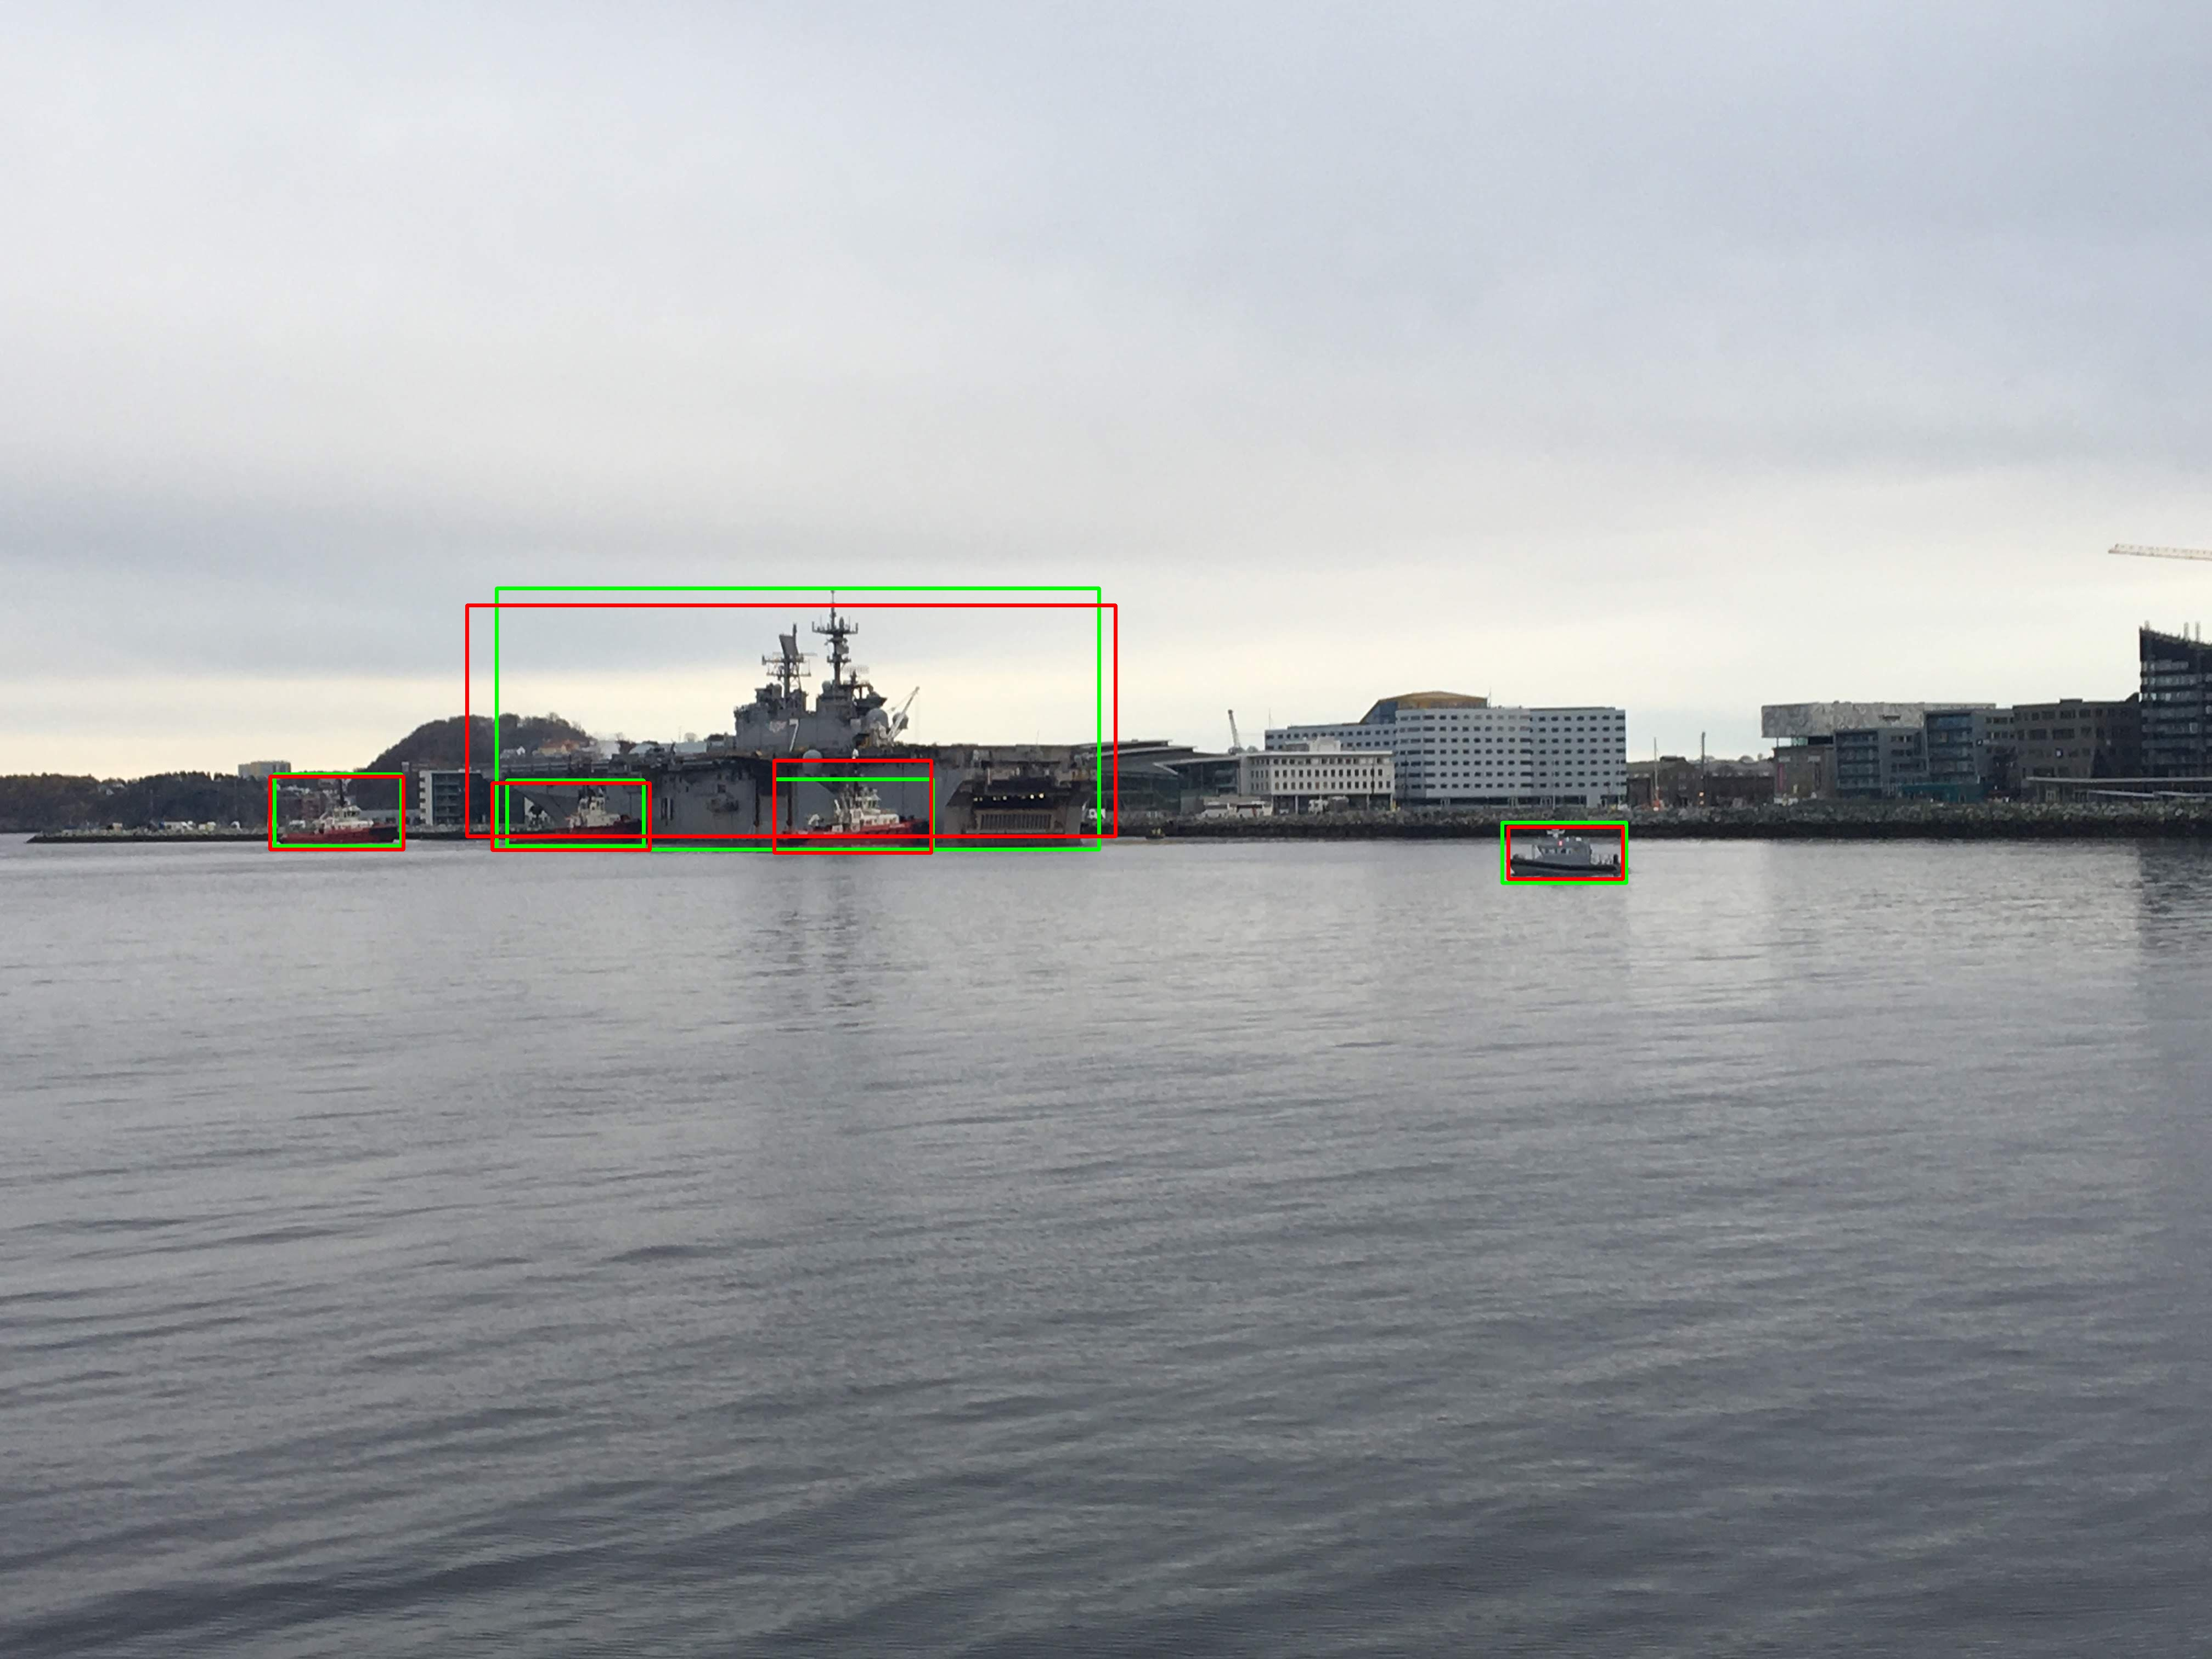
\includegraphics[width=.8\linewidth]{discussion/yolo3_no_build/IMG_2695.jpg}
  %\caption{Three tow boats separated}
  %\label{fig:yolo1_sep}
\end{subfigure}
\caption{Yolo$_{\text{BSMH}}$ fails to detect buildings in the background.}
\label{fig:yolo3_no_build}
\end{figure}

\noindent
The buildings in figure \ref{fig:buildings} and \ref{fig:yolo3_no_build} are in different scales. The results in this project indicate that training on images like the ones in figure \ref{fig:buildings} do not translate well to detecting buildings like the ones in figure \ref{fig:yolo3_no_build}. Still, the idea behind training a detection model on a building dataset was not that it should detect all the buildings in test datasets, but rather learn to not classify buildings as boats. 

\newpage

\section{Labeling}

During labeling of the dataset, the guidelines mentioned in chapter \ref{sec:labeling} was used. Three problems were encountered during the work with this project related to how the boats were labeled

\subsection{Labeling of sail boats}

In figure \ref{fig:yolo3_sailboat} there are examples where sailboats are detected differently. In figure \ref{fig:yolo3_sailboat_whol} the whole sailboat is detected, with mast, in figure \ref{fig:yolo3_sailboat_part} the mast is not detected as a part of the boat. As can be seen in both figure \ref{fig:yolo3_sailboat_whol} and \ref{fig:yolo3_sailboat_part} sailboats are labeled with mast. Thus, the correct detection set by the labeling standards would include the mast, however, to detect the mast may not be necessary for an autonomous vessel. The shape of the sailboat hull is comparable to the hulls of motor boats and also larger ships. By labeling sailboats with the mast, instead of only the hull of the boat, the detector might be less likely to be able to generalize the hull shape. Labeling only the sailboat hull makes the boats more alike, which may make the detector model more certain when classifying. 



\begin{figure}[h!]
\begin{subfigure}{.5\textwidth}
  \centering
  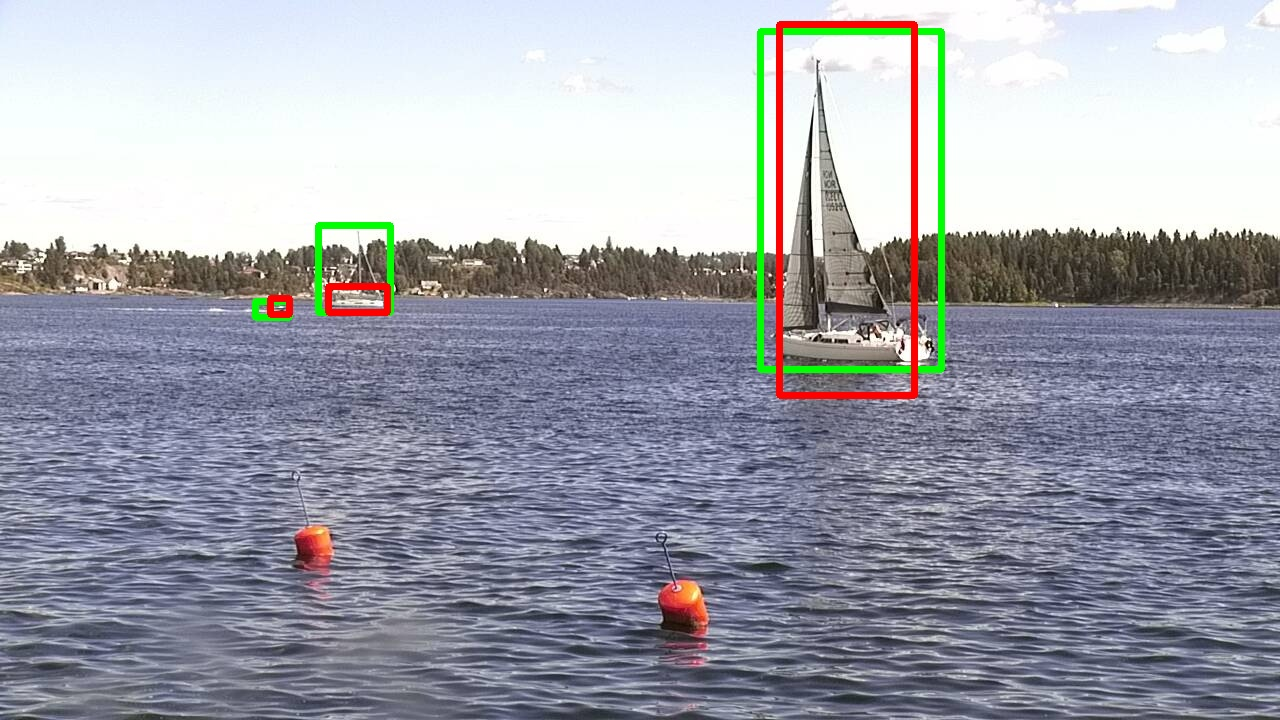
\includegraphics[width=0.8\linewidth]{discussion/sailboat/selected_06_25_frame0349.jpg}
  \caption{Yolo$_{\text{BSMH}}$ detects whole sailboat.}
  \label{fig:yolo3_sailboat_whol}
\end{subfigure}%
\begin{subfigure}{.5\textwidth}
  \centering
  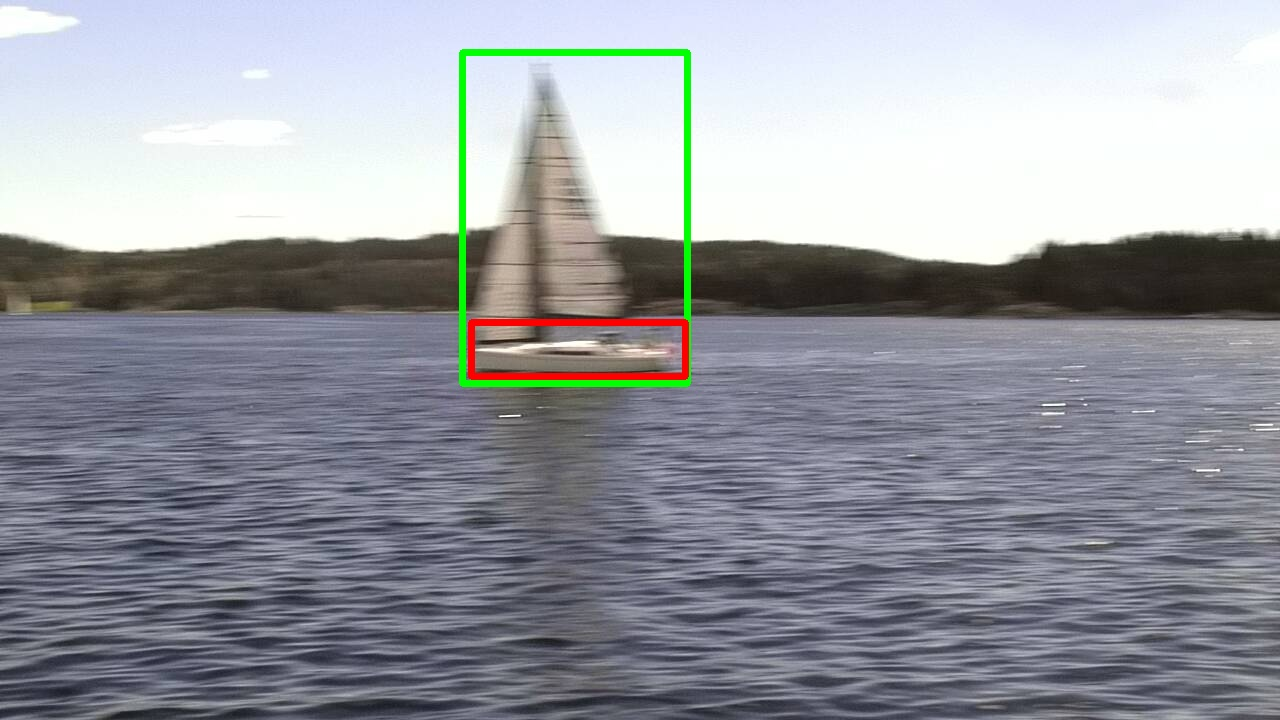
\includegraphics[width=.8\linewidth]{discussion/sailboat/selected_06_25_frame0340.jpg}
  \caption{Yolo detects part of sailboat.}
  \label{fig:yolo3_sailboat_part}
\end{subfigure}
\caption{Yolo$_{\text{BSMH}}$ detects two sailboats differently.}
\label{fig:yolo3_sailboat}
\end{figure}


\subsection{Using several boat classes}
Another option is to train on different boat classes, having one class for motor vessels, sailboats, cargo ships, kayaks and so on. The features of a kayak will be different from a military frigate and trying to classify all these as the same object might confuse the detector. Yet, this would require datasets for each boat class, which would require much more data than what was used in this project.

\subsection{Detecting boat parts}
\label{sec:boat_parts}
The detection models seem to struggle when boats are partly covered by other boats or objects, and will either only detect the foremost boat, or detect the two boats as one large object, as shown in figure \ref{fig:video3}. To be able to correctly classify a boat that is partly covered as a boat, the detection algorithm has to recognize parts of boats as boats. If large parts of a boat are covered, a detector trained on non-covered boats will not robustly detect it. A possible solution could be to train an object detector on parts of boats and post-process the detections into full boat detections. This does not seem like an easy system to implement and would require a massive amount of data. 



\section{Clustered boats}
Both Yolo and SSD have good results when there is a limited amount of boats in the image, and they are separated. When small boats are clustered together, like in figure \ref{fig:yolo3_clutter} both detection algorithms have trouble detecting them. This is not surprising as it is hard to make out the boats individually, also by human assessment. 

\vspace{3mm}
\noindent
For Yolo, there are two main ways of approaching this problem. Either the grid can be resized and that way Yolo can detect smaller objects. This because there will be more cells in the grid, thereby creating more object proposals. The other solution, which might work better in this case, is to identify where there might be clusters and run Yolo on this sub-region of the image. This would require some form of cluster detection, which has been done in \citep{VanEtten}, though on detection of boats in satellite images. 

